\documentclass[a4paper]{article}
\usepackage[paper=a4paper,left=24mm,right=24mm,top=20mm,bottom=20mm]{geometry}

%% Language and font encodings
\usepackage[english]{babel}
%\usepackage[utf8x]{inputenc}
\usepackage{pgfgantt}
\usepackage{rotating}
\usepackage{float}
%\usepackage[english, ngerman]{babel}
\usepackage{graphicx}                               % For includegraphics
\usepackage{wrapfig}                                % For wrapfig environment
\usepackage{paralist}                               % For compactitem 
\usepackage{xcolor}
\usepackage[utf8]{inputenc}
\usepackage{sectsty}
\usepackage{hyperref}
\usepackage{paralist}
\usepackage{booktabs}
\usepackage{tabu}
\usepackage[affil-it]{authblk}
\usepackage[T1]{fontenc}

%% Sets page size and margins

%% Useful packages
\usepackage{amsmath}
%\usepackage{apacite}
\usepackage[colorinlistoftodos]{todonotes}
\input{julia_listings}
\renewcommand\Authfont{\fontsize{14}{14.4}\selectfont}
\renewcommand\Affilfont{\fontsize{12}{14.4}\selectfont}
%Write the title of your project here:
\title{Differentiating sparse matrix operations with reversible programming}
%Here goes your full name
\author{Jie Li}
\affil{Mentors: Jinguo Liu, Jiuning Chen}
\date{\today}

\begin{document}
\maketitle



\section{Project Information}
\subsection{Scheme Description}
Sparse matrices are extensively used in scientific computing, however there is no automatic differentiation package in Julia yet to handle sparse matrix operations yet. This project will utilize the reversible embedded domain-specific language NiLang.jl to differentiate sparse matrix operations by re-writing the sparse functions in Julia base in a reversible style. I will port the generated backward rules to ChainRules.jl as an extension, where ChainRules.jl is the most popular Julia package providing backward rules for automatic differentiation packages. 
\subsection{Time Planning}

This project will be shipped by four (mostly) sequential stages:
\begin{enumerate}[(1)]
    \item Implement low level operations by NiLang.
    \item Carefully test by CI and export chain rules into ChainRules.jl. 
    \item Implement high level operations by NiLang and export chain rules.
    \item Rebase the project on NiLang.Core and merge it into NiLang.jl.
\end{enumerate}

I list the timeline of this project in the form of Gantt chart.
\begin{enumerate}[(1)]
    \item 1st Jul - 31st Jul \quad Implement low level operations by NiLang. 
    \item 1st Aug - 15th Aug   \quad Carefully test by CI and export chain rules into ChainRules.jl.
    \item 15th Sep - 20th Sep \quad  Implement high level operations by NiLang and export chain rules. 
    \item 21st Sep - 30th Sep \quad Rebase the project on NiLang.Core and merge it into NiLang.jl.
\end{enumerate}
\vspace{0.5cm}

\noindent\resizebox{\textwidth}{!}{
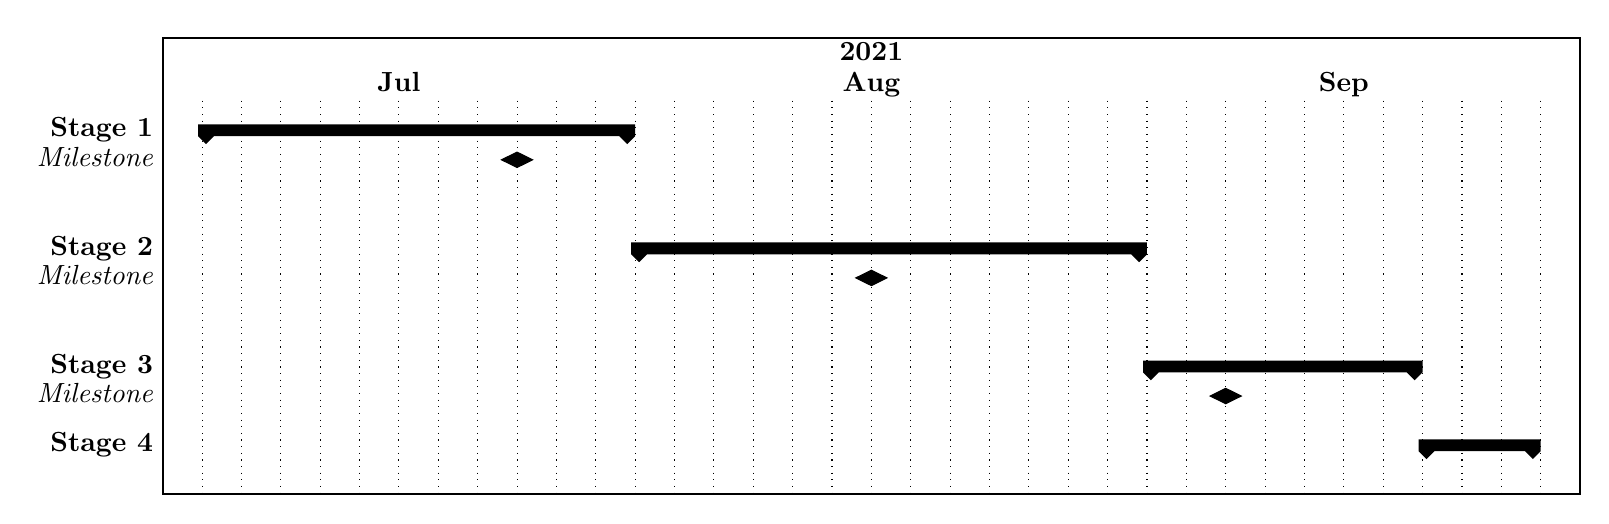
\begin{tikzpicture}[x=.5cm, y=1cm] 
\centering
        \begin{ganttchart}[%Specs
            y unit title=0.4cm,
            y unit chart=0.5cm,
            canvas/.style={fill=none, draw=black, line width=.75pt},
            vgrid,
            title label anchor/.style={below=-1.6ex},
            title left shift=.05,
            title right shift=-.05,
            title height=1,
            title/.style={fill=none},
            title label font=\bfseries,
            bar/.style={fill=barblue},
            incomplete/.style={fill=white},
            progress label text={},
            bar height=0.7,
            group right shift=0,
            group top shift=.6,
            group height=.3,
            group peaks height=.2]{1}{36}

            %labels
            \gantttitle{2021}{36}\\
            \gantttitle{Jul}{12}
            \gantttitle{Aug}{12}
            \gantttitle{Sep}{12}
            \\

            % Parameter Selection
            \ganttgroup{Stage 1}{2}{12}\\ %elem0
            %\ganttbar[progress=0]{sub-objective}{2}{18}\\
            \ganttmilestone{Milestone}{9}\\\\

            % Testing equipment
            \ganttgroup{Stage 2}{13}{25}\\ %elem0
            %\ganttbar[progress=0]{Bar}{2}{18}\\
            \ganttmilestone{Milestone}{18}\\\\

            % Testing
            \ganttgroup{Stage 3}{26}{32}\\ 
            %\ganttbar[progress=0]{Bar}{19}{35}\\
            %\ganttbar[progress=0]{Bar}{19}{35}\\
            \ganttmilestone{Milestone}{27}\\
            %\ganttmilestone{Milestone}{35}\\

            % Algorithm Development
            \ganttgroup{Stage 4}{33}{35}\\ 
            %\ganttbar[progress=0]{Bar}{28}{35} \\

            %relations 
            %\ganttlink{elem2}{elem6}
            %\ganttlink{elem5}{elem6}
            %\ganttlink{elem9}{elem11}

        \end{ganttchart}
    \label{fig:Gantt2014}
\end{tikzpicture}}  

\vspace{0.5cm}  

\section{Project Schedule}
\subsection{The Accomplished Work}
In the first phase, we unified the sparse matrix operations and established 
the whole pipeline for automatic differentiation in the project.
\paragraph{Unify Sparse Matrix Operations} 
Initial goal of the project is to implement sparse matrix operators and generate corresponding 
automatic differentiation compared with Pytorch. However, as mentioned in 
\href{https://github.com/pytorch/pytorch/issues/45897}{Issue in Pytorch}, the users have 
difficulties in choosing the matmul function they need since the functionalities of these functions 
is not independent to each other. I outlined the sparse matrix operators to be implemented as follows. 
\begin{lstlisting}[language=Julia]
    imul!(C::StridedVecOrMat, A::AbstractSparseMatrix, B::DenseInputVecOrMat, alpha::Number, beta::Number)
    imul!(C::StridedVecOrMat, xA::Adjoint{<:Any,<:AbstractSparseMatrix}, B::DenseInputVecOrMat, alpha::Number, beta::Number)
    imul!(C::StridedVecOrMat, X::DenseMatrixUnion, A::AbstractSparseMatrix, alpha::Number, beta::Number)
    imul!(C::StridedVecOrMat, X::Adjoint{<:Any,<:DenseMatrixUnion}, A::AbstractSparseMatrix, alpha::Number, beta::Number)
    imul!(C::StridedVecOrMat, X::DenseMatrixUnion, xA::Adjoint{<:Any,<:AbstractSparseMatrix}, alpha::Number, beta::Number)
    idot(r::T, A::SparseMatrixCSC{T},B::SparseMatrixCSC{T}) where {T}
    idot(r, x::AbstractVector, A::AbstractSparseMatrix{T1}, y::AbstractVector{T2}) where {T1, T2}
    idot(r, x::SparseVector, A::AbstractSparseMatrix{T1}, y::SparseVector{T2}) where {T1, T2}
    i_spmatmul(A::SparseMatrixCSC{Tv, Ti}, B::SparseMatrixCSC{Tv, Ti}) where {Tv, Ti}
\end{lstlisting}
It is considered to be a suitable unification since the protype of \textit{imul!} is 
gaxpy operation in numerical maths, which is a generalization to matrix multiplication.
Besides, Julia's type system and dot operations are also taken into account.      
So far, seven of the methods have been implemented and all tests have passed (both in local and CI).
For more detailed implementations and test cases, check for this 
\href{https://github.com/jieli-matrix/NiSparseArrays.jl/tree/dev}{branch} and  
the test converage is over 80\%.  

\paragraph{Generate Automatic Differentiation Rules}
Ultimate goal of the project is to provide Automatic Differentiation (AD) rules on sparse 
matrix operators generated by NiLang. To outline the development in the AD section, 
one should consider how to generate rules and how to test the accuracy of rules. 
There are many choices to do these and I finally establish the pipeline for AD part in this project as follows.
\begin{enumerate}[(1)]
    \item Write rrule in support of ChainRulesCore.jl. Rules would be generated by NiLang.
    \item Test rrule in support of ChainRulesTestUtils.jl. 
    \item Provide the passed rules to ChianRules.jl. 
\end{enumerate}  
The pipeline is also consistent with the idea metioned in 
\href{https://raw.githack.com/oxinabox/ChainRulesJuliaCon2020/main/out/build/index.html#1}{JuliaCon 2020} by Lyndon White.
So far, I generate AD rules by NiLang and ChainRulesCore and test rules by ChainRulesTestUtils
under the help of mentors. For more detailed implementations and test cases, check for this 
\href{https://github.com/jieli-matrix/NiSparseArrays.jl/tree/master}{branch} and  
the test converage is over 80\%.

\subsection{Problem and Solution}
It is the most difficult project for me so far since I am totally new to NiLang and AD. 
For NiLang, it would be easy for me to write the code in syntax but the high performance 
couldn't be ensured. For AD, I even couldn't figure out how AD works in computation theory 
before but I need to generate AD rules in this project. 
\subsubsection{Problems on NiLang Section}
\paragraph{Performance Gap} In benchmark tests, we found the implementation of matrix multiplication between 
Adjoint sparse matrix and dense matrix is about 2x slower than the one in Julia base. Finally,
we found the reason by profiling the program.
\begin{lstlisting}[language=Julia]
julia> @profile for i=1:100 imul_v1!(C, A', b, 1.0, 1.0) end

julia> Profile.print(mincount=20; format=:flat);
 Count  Overhead File                               Line Function
 =====  ======== ====                               ==== ========
  1900         0 @Base/Base.jl                        39 eval
  1900         0 REPL[42]                              1 macro expansion
   217       217 @Base/array.jl                      802 getindex
  1126      1126 @Base/array.jl                      841 setindex!
  1900         0 @Base/boot.jl                       360 eval
  1900         0 @Base/essentials.jl                 708 #invokelatest#2
  1900         0 @Base/essentials.jl                 706 invokelatest(::Any)
    30        30 @Base/float.jl                      332 *
   242       242 @Base/float.jl                      326 +
  1900         0 @Base/logging.jl                    603 with_logger
  1900         0 @Base/logging.jl                    491 with_logstate(f::Function, logstate::Any)
   255       255 @Base/promotion.jl                  410 ==
   263         8 @Base/range.jl                      674 iterate
  1900         0 @Base/task.jl                       411 (::VSCodeServer.var"#53#54")()
   272         0 @NiLangCore/src/Core.jl             232 #_#36
   272         0 @NiLangCore/src/Core.jl             232 PlusEq
   263         0 @NiSparseArrays/src/linalg.jl        47 imul_v1!(C::Matrix{Float64}, xA::LinearAlgebra.Adjoint{Float64, SparseMatrixCSC{Float64, Int64}}, B::Matrix{Fl...
   247         0 @NiSparseArrays/src/linalg.jl        48 imul_v1!(C::Matrix{Float64}, xA::LinearAlgebra.Adjoint{Float64, SparseMatrixCSC{Float64, Int64}}, B::Matrix{Fl...
  1375         0 @NiSparseArrays/src/linalg.jl        50 imul_v1!(C::Matrix{Float64}, xA::LinearAlgebra.Adjoint{Float64, SparseMatrixCSC{Float64, Int64}}, B::Matrix{Fl...
  1900         0 @VSCodeServer/src/eval.jl            34 macro expansion
  1900         0 @VSCodeServer/src/repl.jl           124 (::VSCodeServer.var"#68#70"{Module, Expr, REPL.LineEditREPL, REPL.LineEdit.Prompt})()
  1900         0 @VSCodeServer/src/repl.jl           123 (::VSCodeServer.var"#69#71"{Module, Expr, REPL.LineEditREPL, REPL.LineEdit.Prompt})()
  1900         0 @VSCodeServer/src/repl.jl           157 repleval(m::Module, code::Expr, #unused#::String)
  1900         0 @Profile/src/Profile.jl              28 top-level scope
Total snapshots: 3800

\end{lstlisting}

The setindex operation takes to much time. It is related to "trait" of NiLang that it assigns an input variable back to the array.
If we copy the element out first to a scalar, it would ease the problem. After correcting the problem, the performance gap is constrained 
into 1.2 times. For more detailed dicussion on this problem, check for this \href{https://github.com/jieli-matrix/NiSparseArrays.jl/pull/15}{PR}.

\paragraph{Gustavson Sparse Matrix Multiplication} Different from traditional gaxp operations,
Gustavson algorithm is applied in sparse matrix multiplication. One of the high efficiency comes from 
the estimate on the number of non-zero elements in $\mathbf{C}$. However, it is hard to define the reversible 
operations on the extension and shrink of the memory in NiLang. We pended the problem in \href{https://github.com/jieli-matrix/NiSparseArrays.jl/issues/14}{this issue} now and 
left it for further exploration.  


\subsubsection{Problems on AD Section}

\paragraph{Establish the whole pipeline} As I mentioned before, one should consider how to generate rules and how to test the accuracy of rules. 
In fact, I completed the implementation of sparse matrix operators much earlier before August. However, I am new to AD both in theory and techniques
and spend much time on AD part. At first, I wrote the tests on calculating the jacobian matrix using ForwardDiff. I realized I didn't care the jacobian 
matrix but rrule and the tests on rrule until this week. However, I still don't know to choose which package to test the accuracy of rules in Julia since there are 
many choices provided in \href{https://juliadiff.org/ChainRulesCore.jl/stable/#Example-of-using-ChainRules-directly}{scalar cases} in ChainRules.jl.
I'd like to thank mentors for pointing the problem and recommending ChainRulesCore / ChainRulesTestUtils to do this.

\paragraph{How to complete an unfamiliar project in a short time} In this part, I'd like to mention a general problem students
involed in OSPP projects would face: Students learn the basics or maybe the outdated knowledge in school but they would try to complete 
the project using the techniques / theory they never heard before. Take myself experience as an example. If one wants to learn about a new feild, it usually begins with 
a classical tutorial or a friendly course. However, I don't have so much time to learn AD since OSPP
is a three-month project not a course. I read papers about ForwardDiff and Tapenade recommended by mentors;
I read blogs and watched open talks on AD in Machine Learning and Scientific Computation; I watched the AD talk 
on JuliaCon times by times since people commented it is not newcomer-friendly. Now I could summarize the experience 
as follows: \textit{Differentiation is originally a pure mathematical concept, and we could make it Automatic by 
Tangent Mode and Adjoint Mode. Then AD is extended to the computaion concept, we want to calculate the differentiation of 
a program. Many techniques have been proposed such as operator overloading, source code transformation and so on. 
Julia have many AD packages under development like Zygote, ForwardDiff, etc. It would cost one much time to 
consider the relationship between the AD theory and packages but it would also be exciting.} 
So what could we learn from the example? We shouldn't expect the candidate to be the related
expert or researcher. The open source community could release more good first issues and draw a 
more systematic introduction to the framework and techniques in the project. The OSPP students are also encouraged to share their 
experience and help newcomers to join in the community.   

\subsection{Subsequent Work Arrangement}
In the subsequent, we would focus on the four main parts:
\begin{enumerate}[(1)]
    \item Implementation of high-level operators.
    \item Generate rrules and test the accuracy for all operators.
    \item Rebase the project on NiLang.Core and merge it into NiLang.
    \item Explore the possible solutions for pending problems like Gustavson algorithm.
\end{enumerate}


\bibliographystyle{plain}
\bibliography{refs}

\newpage
\input{Preamble_CV.tex}
\MyName{Jie Li}

\sepspace

%%% Personal details--------------------------------------------------------------------------

\SimpleEntry{\textbf{Github}: \href{https://github.com/jieli-matrix}{https://github.com/jieli-matrix}}
\SimpleEntry{\textbf{Website}: \href{https://jieli-matrix.github.io/}{https://jieli-matrix.github.io/}}
\SimpleEntry{\textbf{Email}: li\_j20@fudan.edu.cn}

%%% Education---------------------------------------------------------------------------------
\NewPart{Education}

\TimeEntryFocus{9.2020 - 6.2023}
{Master of Applied Mathematics }{at Fudan University}
{Supervised by Young PI \href{https://scholar.google.com/citations?user=bLERs80AAAAJ&hl=zh-CN}{Weiyang Ding}\\
Focus on Numerical Optimization and Matrix Computation}
\sepspace

\TimeEntry{9.2016 - 7.2020}
{Bachelor of Mathematics and Applied Mathematics}{at Lanzhou University}
\sepspace


%%% Skills and Qualifications --------------------------------------------------------------
\NewPart{Skills and Qualifications}
\NewSubPart{Programming Languages}
\TitleEntry{Advanced skills}{Python, Julia, Matlab}
\TitleEntry{Basic skills}{Git, Linux, Cpp}

\NewSubPart{Languages}
\TitleEntry{Native}{Chinese}
\TitleEntry{Advanced}{English (TOEFL:94 CET-4:632 CET-6:571)}

%%% Work experience------------------------------------------------------------------------
\NewPart{internship experience}
\TimeEntryDesc{10.2019 - 12.2019}{NLP Researcher in Core Development Platform}{at \href{https://www.iflytek.com/}{iFLYTEK}}
{\begin{compactitem}
    \item Automatic Pipeline on Senior High School Math Homework 
    \item Code Implementation of  \href{https://arxiv.org/abs/1911.06557}{Multi-Label Learning with Deep Forest}
\end{compactitem}
}



%%% Skills and Qualifications --------------------------------------------------------------
\NewPart{Projects}
\TimeEntryDesc{5.2021 - now}{Lowranksvd.jl}{ \href{https://github.com/jieli-matrix/Lowranksvd.jl/tree/dev}{Lowranksvd.jl}}
{\begin{compactitem}
    \item Algorithm 4.4 from \href{https://arxiv.org/abs/0909.4061}{Halko et al.} implemented by Julia with all CI tests passing.
    \item Algorithm 5.1 from \href{https://arxiv.org/abs/0909.4061}{Halko et al.} implemented by Julia with all CI tests passing.
\end{compactitem}
}

\TimeEntryDesc{4.2020}{CPUPredict}{\href{https://github.com/VealM/CPUPredict}{CPUPredict}}
{
    Time series prediction of the CPU's usage rates.  

    This project won the third place in Elastic Cloud College Challenge held by ALibaba.
}

\NewPart{Contests}
\TimeEntryDesc{11.2020}{Brain-Inspired Intelligence Contests held by Fudan University}{\quad}{
    \textbf{Efficent information encoding and energy efficiency in E/I balanced neuronal networks}  

    Numerical Simulation for E/I balanced neuronal networks.  
      
    I won the third place in the contest. 
}



\end{document}